\documentclass[11pt,letterpaper,boxed]{pset}

\usepackage[margin=0.75in]{geometry}
\usepackage{ulem}

\name{Name: \rule{2.5cm}{0.15mm}}
\assignment{Box \# \rule{1.5cm}{0.15mm}}
\class{MATH060 HW10}
\duedate{04 June 2019}

\begin{document}

    \problemlist{MATH060 HW10}
    \begin{center}
    	6.1: 2, 9, 21, 31, 34, 40 \\
    	6.2: 4
    \end{center}
    
    \begin{problem} [6.1.2]
    	Calculate $\int_\textbf{x} f \textrm{ } ds$, where $f$ and $\textbf{x}$ are:
    
    	\[f(x,y,z)=xyz,\textrm{ } \textbf{x}(t) = (t, 2t, 3t), \textrm{ } 0 \leq t \leq 2\]
    
    \end{problem}
    \newpage
    
    
    \begin{problem} [6.1.9]
    	Find $\int_\textbf{x} \textbf{F} \cdot d\textbf{s}$, where the vector field $\textbf{F}$ and the path $\textbf{x}$ are:
    
    	\[\textbf{F} = (y+2)\textbf{i} + x\textbf{j}, \textrm{ } \textbf{x}(t) = 
    		(\textrm{sin}t, -\textrm{cos}t), \textrm{ } 0 \leq t \leq \pi / 2\]
    
    \end{problem}
    \newpage
    
    
    \begin{problem} [6.1.21]
    	Let $\textbf{F} = (x^2 + y)\textbf{i} + (y - x)\textbf{j}$ and consider the two paths
    	
    	\begin{align*}
    	    \textbf{x}(t) &= (t,t^2), \textrm{ } 0 \leq t \leq 1 \\
    	    \textbf{y}(t) &= (1-2t, 4t^2-4t+1), \textrm{ } 0 \leq t \leq \frac12
    	\end{align*}
    
        \begin{enumerate} [(a)]
            \item Calculate $\int_\textbf{x} \textbf{F} \cdot \textrm{ } d\textbf{s}$ and $\int_\textbf{y} \textbf{F} \cdot \textrm{ } d\textbf{s}$.
    		\item By consider the image curves of the paths \textbf{x} and \textbf{y}, discuss your answers in part (a).
        \end{enumerate}
    	
    \end{problem}
    \newpage
    
    
    \begin{problem} [6.1.31]
    	Evaluate $\int_C yz\textrm{ } dx - xz\textrm{ }dy + xy\textrm{ }dz$, where $C$ is the line segment from (1, 1, 2) to (5, 3, 1).
    \end{problem}
    \newpage
    
    
    \begin{problem} [6.1.34]
    	Tom Sawyer is whitewashing a picket fence. The bases of the fenceposts are arranged in the $xy$-plane as the quarter circle $x^2 + y^2 = 25$, $x$, $y \geq 0$, and the height of the fencepost at point $(x, y)$ is given by $h(x, y) = 10 - x - y$ (units are feet). Use a scalar line integral to find the area of one side of the fence.
    
    \end{problem}
    
    \begin{minipage}[t]{0.5\textwidth}
    	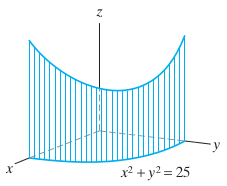
\includegraphics[width=\textwidth]{fence.png}
    	Figure 1: The base of the fence is the quarter circle 
    		$x^2 + y^2 = 25$, $x$, $y \geq 0$
    \end{minipage}
    \newpage
    
    
    \begin{problem} [6.1.40]
        You are currently located 20 miles due east of Cleveland and are attempting to drive to a point 20 miles due west of Cleveland. Further suppose that if you are $s$ miles from the center of Cleveland, you can drive at a rate of at most $v(s) = 2s + 20$ miles per hour.
        \bigskip
    	
    	\begin{enumerate} [(a)]
    	    \item How long will the trip take if you drive on a straight-line path directly through Cleveland at the maximum speed possible?
    	    \item How long will the trip take if you avoid the middle of the city by driving along a semicircular path with Cleveland at the center at the maximum speed possible?
    	    \item Repeat parts (a) and (b), this time using $v(s) = (s^2 /16) + 25$ miles per hour as the maximum speed that you can drive.
    	\end{enumerate}
    
    \end{problem}
    \newpage
    
    
    \begin{problem} [6.2.4]
    	Verify Green's theorem for the given vector field 
    
    	\[\textbf{F} = M(x,y)\textbf{i} + N(x,y)\textbf{j}\]
    
    	and region $D$ by calculating both 
    
    	\[\oint_{\partial D} M\textrm{ } dx + N\textrm{ } dy \textrm{  and } \iint_D (N_x - M_y)dA.\]
    
    	$\textbf{F} = (2y)\textbf{i} + (x)\textbf{j},$ $D$ is the semicircular region $x^2+y^2 \leq a^2$, $y \geq 0$.
    
    \end{problem}
    \newpage

\end{document}